% v2u figure snippets, include from ieee_publication_assets/latex
% Requires graphicx
\begin{figure}[t]
\centering
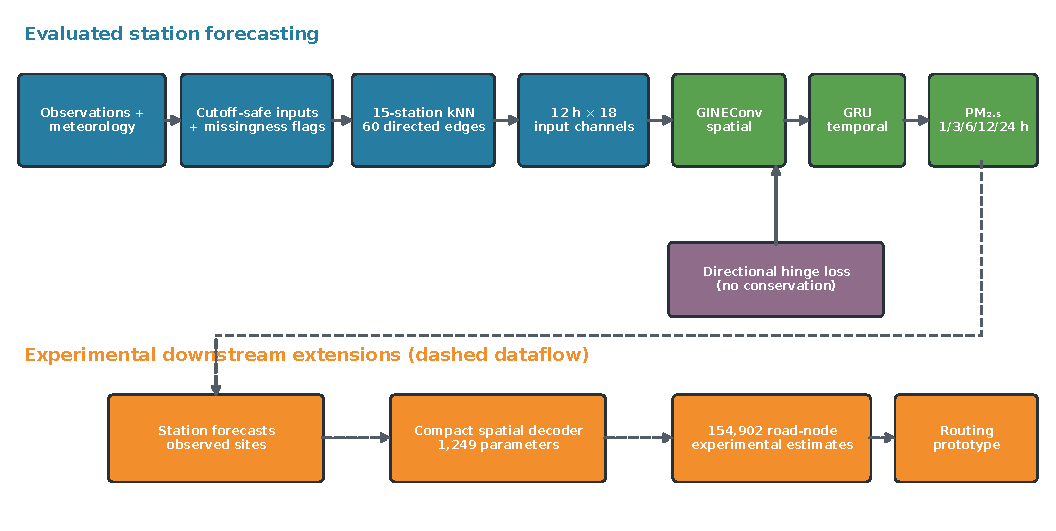
\includegraphics[width=\columnwidth]{../figures/F01_architecture/F01_corrected_architecture.pdf}
\caption{Solid: evaluated station forecasting and loss. Dashed: experimental decoder and routing dataflow. Road GNN training and mass conservation are not shown because neither was established.}
\label{fig:f01_corrected_architecture}
\end{figure}

\begin{figure*}[t]
\centering
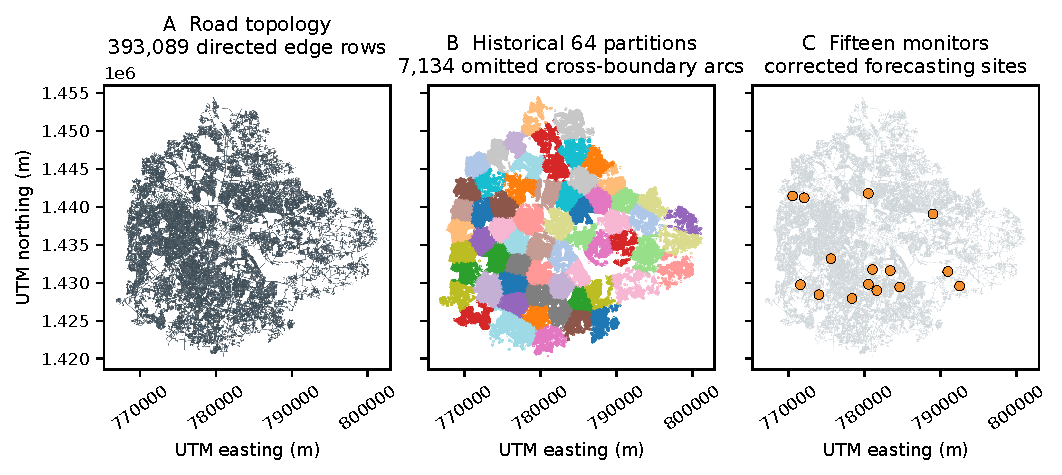
\includegraphics[width=\textwidth]{../figures/F02_graph_partitions/F02_bengaluru_graph.pdf}
\caption{Stored UTM graph and partition IDs; 154,902 nodes. The corrected forecasting model was evaluated on a separate 15-station, 60-edge kNN graph, not on the road graph. Arc and edge-row counts have different preprocessing semantics.}
\label{fig:f02_bengaluru_graph}
\end{figure*}

\begin{figure*}[t]
\centering
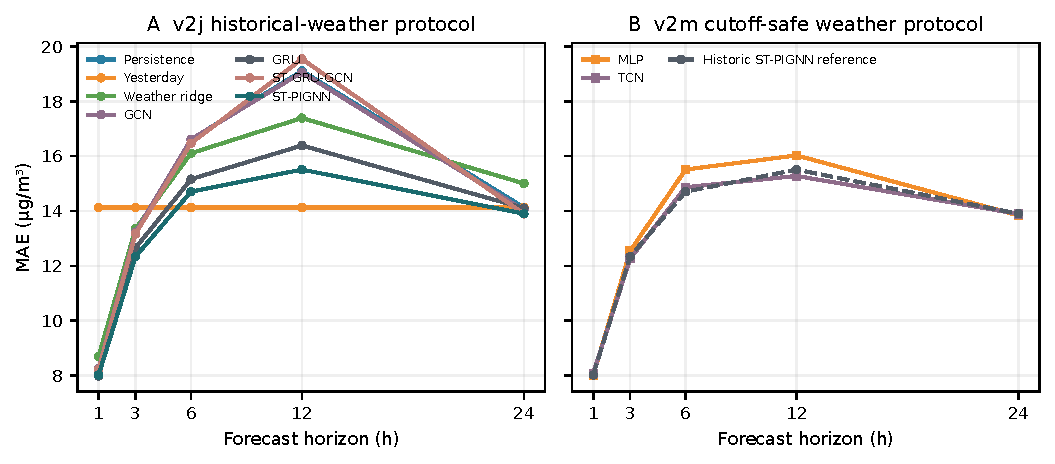
\includegraphics[width=\textwidth]{../figures/F03_forecasting_benchmarks/F03_multi_horizon_mae.pdf}
\caption{Five forecast horizons; 14,583 saved evaluation pairs per horizon. v2j ST-PIGNN and v2m MLP/TCN used different weather aggregation and are not identical-input architecture ablations. Negative and unfavorable results are retained.}
\label{fig:f03_multi_horizon_mae}
\end{figure*}

\begin{figure*}[t]
\centering
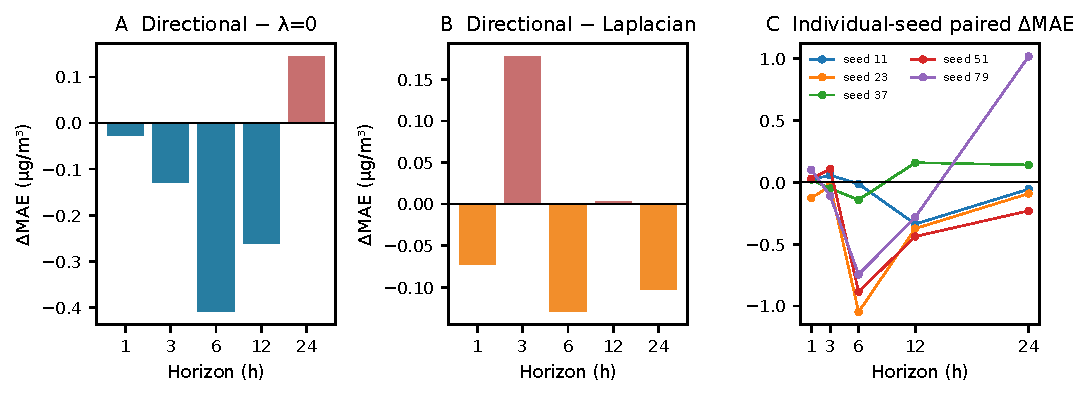
\includegraphics[width=\textwidth]{../figures/F04_physics_ablations/F04_directional_ablation.pdf}
\caption{Negative ΔMAE favors directional regularization. Panels A/B are five-seed ensemble differences; C shows individual-seed paired differences. No physical-specificity or mass-conservation inference follows. Multiplicity and seven-day block sensitivity are reported in T03.}
\label{fig:f04_directional_ablation}
\end{figure*}

\begin{figure*}[t]
\centering
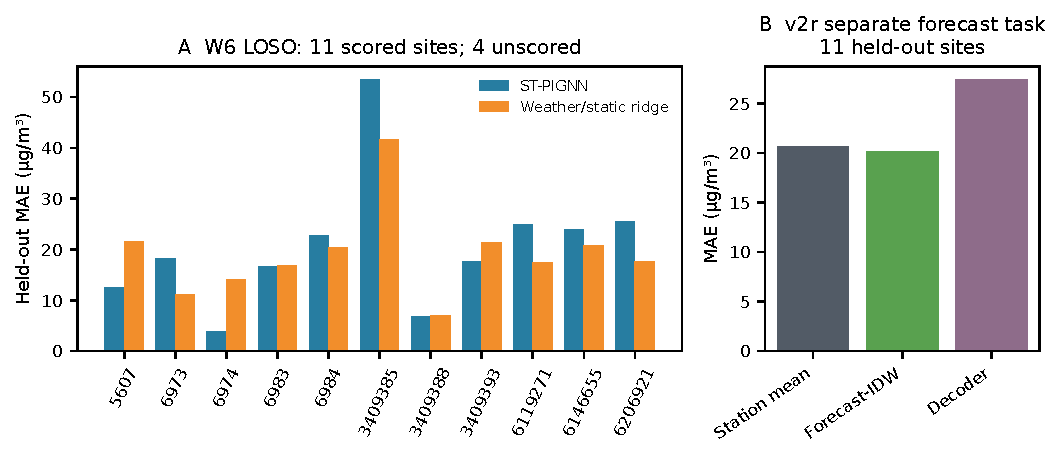
\includegraphics[width=\textwidth]{../figures/F05_spatial_validation/F05_spatial_holdouts.pdf}
\caption{W6 pooled MAE: ST-PIGNN 22.314 versus ridge 20.624 $\mu$g/m³; 11 scored stations, four without test observations. v2r is a separate forecast population: decoder 27.360, forecast-IDW 20.154, station mean 20.634 $\mu$g/m³. Timestamps are not independent spatial sites.}
\label{fig:f05_spatial_holdouts}
\end{figure*}

\begin{figure*}[t]
\centering
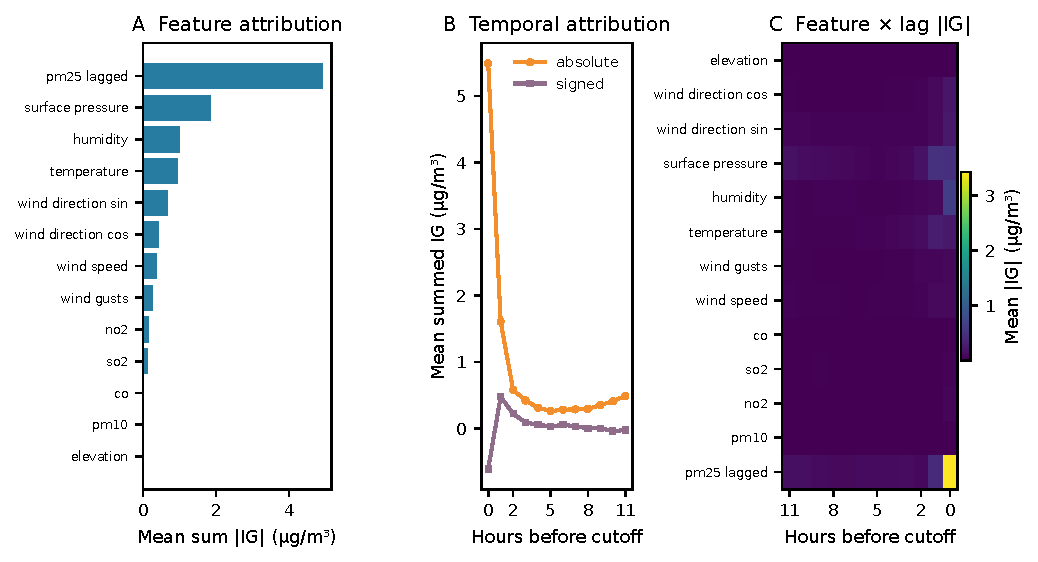
\includegraphics[width=\textwidth]{../figures/F06_captum_explainability/F06a_v2c_h1.pdf}
\caption{Real saved attribution tensors, primary training-mean baseline, 45 attributed records, 12 input hours. Mean absolute and signed IG are separate. Maximum completeness |delta| 2.1e-05 $\mu$g/m³; wrapper error 4.6e-05 $\mu$g/m³. IG is baseline-relative sensitivity, not causality or physics proof. Integration-step count is documented in source methodology.}
\label{fig:f06a_v2c_h1}
\end{figure*}

\begin{figure*}[t]
\centering
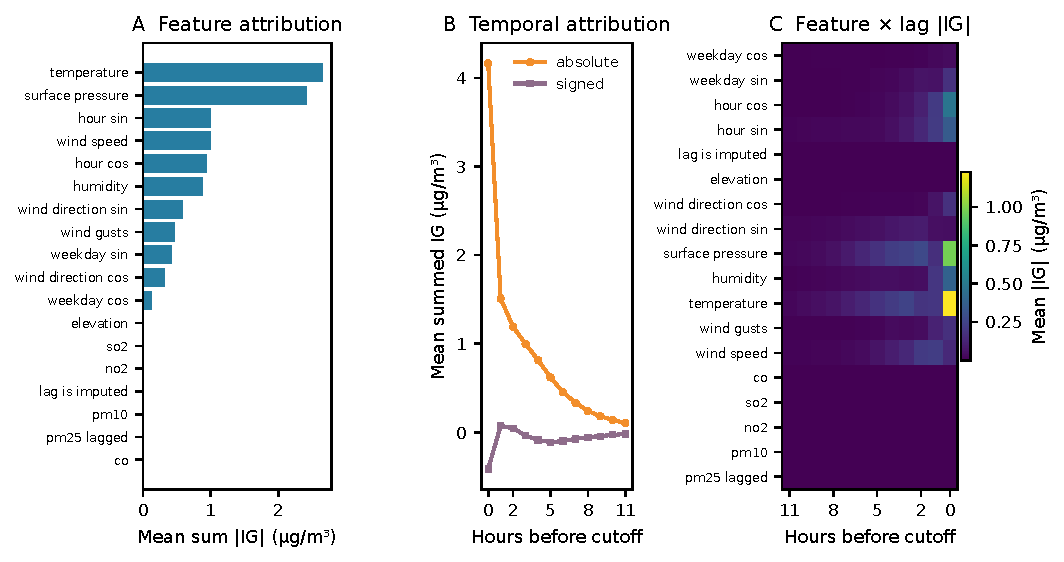
\includegraphics[width=\textwidth]{../figures/F06_captum_explainability/F06b_v2r_h6.pdf}
\caption{Real saved attribution tensors, primary training-mean baseline, 9 attributed records, 12 input hours. Mean absolute and signed IG are separate. Maximum completeness |delta| 7.8e-06 $\mu$g/m³; wrapper error 7.6e-06 $\mu$g/m³. IG is baseline-relative sensitivity, not causality or physics proof. Integration-step count is documented in source methodology.}
\label{fig:f06b_v2r_h6}
\end{figure*}

\begin{figure*}[t]
\centering
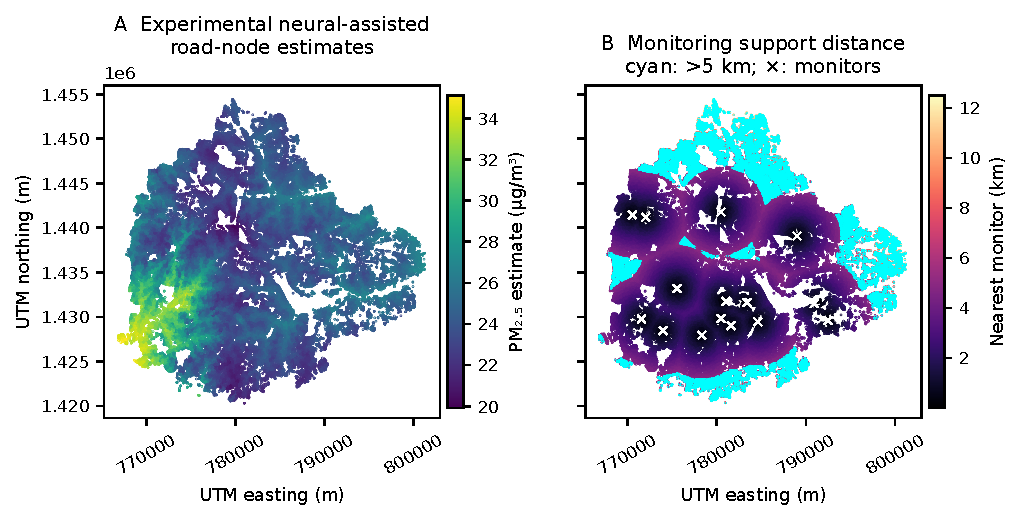
\includegraphics[width=\textwidth]{../figures/F07_citywide_estimation/F07_citywide_snapshot.pdf}
\caption{Earliest frozen origin, 2025-10-08 07:00 UTC, six-hour forecast; 154,902 saved node values without added smoothing. Station forecaster uses 15-station graph; road values use separate 1,249-parameter decoder. Decoder underperformed simple spatial controls; roadside accuracy is unvalidated. 19.45\% of nodes lie >5 km from a monitor; 60.58\% are outside the monitor convex hull.}
\label{fig:f07_citywide_snapshot}
\end{figure*}

\begin{figure*}[t]
\centering
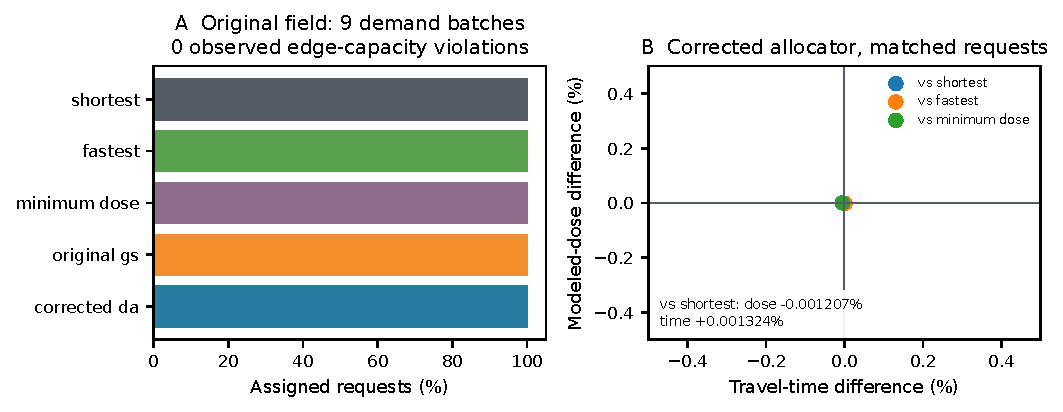
\includegraphics[width=\textwidth]{../figures/F08_routing_evaluation/F08_routing_tradeoff.pdf}
\caption{Original concentration scenario; same nine frozen demand batches, 252 requests per method. Corrected allocator and original matcher assigned all in this low-load case; zero shared-edge violations and maximum utilization about 5.405\%. Corrected versus shortest: −0.001207\% modeled dose and +0.001324\% travel time. Axes intentionally span ±0.5\%. This is modeled dose, not measured exposure reduction or classical matching stability.}
\label{fig:f08_routing_tradeoff}
\end{figure*}

\begin{figure*}[t]
\centering
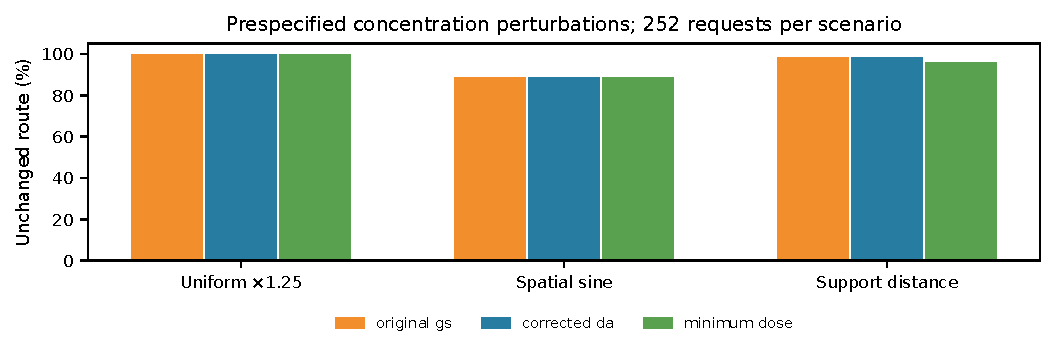
\includegraphics[width=\textwidth]{../figures/F08_routing_evaluation/F08b_routing_sensitivity.pdf}
\caption{Three frozen perturbations relative to the original field; 252 requests each. Bars show route identity stability, not calibrated exposure uncertainty. Assignment stability was 100\% and declared edge-capacity violations zero in saved scenarios. No measured human exposure validation.}
\label{fig:f08b_routing_sensitivity}
\end{figure*}
